\chapter{گراف عامل در رباتیک} \label{sec:appendix1}

\section{تئوری}

در زمینه رباتیک و SLAM، گراف‌های عامل ابزارهای قدرتمندی برای تخمین بهینه حالت هستند. در این پایان‌نامه، ما نیز از این ابزار به عنوان یک چارچوب مؤثر برای شناسایی پارامترها استفاده می‌کنیم. در این بخش، مروری کوتاه بر نظریه‌ها و اصول پشت این روش ارائه می‌دهیم. در اینجا، مفاهیم را در زمینه تخمین حالت توضیح می‌دهیم.

در رباتیک، ترکیب حسگرها می‌تواند به عنوان یک مسئله استنتاج بیزی به شرح زیر فرمول‌بندی شود:
\begin{equation} \label{eq:MAP}
	X^{MAP} = \arg\max_X p(X|Z) = \arg\max_X \frac{p(Z|X)p(X)}{p(Z)}
\end{equation}

که در آن \(Z\) و \(X\) به ترتیب نشان‌دهنده مشاهدات توسط حسگرها و حالت‌های سیستم هستند. تخمین بیشینه پسین
\footnote{\lr{Maximum A Posteriori (MAP)}}
 از حالت‌ها، \(X^{MAP}\)، که نتیجه ترکیب است، از طریق بیشینه‌سازی توزیع پسین \(p(X|Z)\) با استفاده از الگوریتم درست‌نمایی بیشینه
\footnote{\lr{Maximum Likelihood (ML)}}
بدست می‌آید. در این فرمول‌بندی، \(p(Z|X)\) تابع احتمال است که مدل مشاهده حسگرها را نشان می‌دهد، در حالی که \(P(X)\) دانش پیشین از حالت سیستم است. همانطور که در ادامه خواهیم دید، در یک سیستم دینامیکی، این دانش پیشین با استفاده از تابع تحول حالت مدل‌سازی می‌شود.

اگر فرض کنیم \(X\) یک فرایند تصادفی مارکوفی است و \(p(Z|X)\) و \(p(X)\) توزیع‌های نرمال باشند، الگوریتم $ML$ به یک مسئله کمینه مربعات
\footnote{\lr{Least Square (LS)}}
 منجر می‌شود.  حال سیستم غیرخطی زیر را در نظر می‌گیریم:
\begin{equation}
	X_{k+1} = f(X_k, u_k) + w(k), \text{~~~~~~~~~~~~~~~~} z_k = h(X_k) + v(k)
\end{equation}


که در آن \(f(X)\) و \(h(X)\) به ترتیب مدل‌های سیستم و اندازه‌گیری هستند. علاوه بر این، \(v(k)\) و \(w(k)\) نویز گاوسی افزایشی با کوواریانس‌های \(R\) و \(Q\) هستند که به ترتیب نویز اندازه‌گیری و عدم قطعیت مدل را نمایش می‌دهند. بردار \(u_k\) ورودی اختیاری به سیستم است و \(X\) حالت‌های سیستم است. تابع احتمال ممکن است به صورت زیر نوشته شود:
\begin{equation} \label{eq:Gauess_Dis_h}
	p(z|x) = \mathcal{N}(z; h(x), R) = \frac{1}{\sqrt{2\pi R}} \exp \left\{ -\frac{1}{2} \| h(x) - z \|_R^2 \right\}
\end{equation}

این شهود وجود دارد که وقتی حالت \(X\) است، انتظار داریم مشاهده \(h(x)\) باشد. بنابراین،
اندازه‌گیری‌های \(z\) که بسیار متفاوت از \(h(x)\) هستند، کمتر احتمال دارد که رخ دهند. علاوه بر این،
هر چه حسگر دارای نویز کمتری باشد، می‌توانیم با اطمینان بیشتری در مورد این انتظار صحبت کنیم. این
شهود در معادله فوق با استفاده از یک تابع توزیع گاوسی مدل‌سازی شده است که
مرکز آن در \(h(x)\) و واریانس \(R\) است.

از طرف دیگر، توزیع پیشین \(p(X)\) انتظار ما از حالت جدید را بدون داشتن اطلاعاتی به‌جز تخمین قبلی نشان می‌دهد. این دانش از
درک ما از سیستم دینامیکی ناشی می‌شود، که در این حالت، با تابع \(f(X)\)
در معادله
\ref{eq:Gauess_Dis_F}
 نمایش داده می‌شود. بنابراین، مشابه تابع احتمال، توزیع پیشین نیز ممکن است
با استفاده از چگالی گاوسی زیر مدل‌سازی شود:
\begin{equation} \label{eq:Gauess_Dis_F}
	p(x_{k+1}|x_k, u_k) = \frac{1}{\sqrt{2\pi Q}} \exp \left\{ -\frac{1}{2} \| f(x_k, u_k) - x_{k+1} \|_Q^2 \right\}
\end{equation}

اکنون، با توجه به این چگالی‌ها، الگوریتم ML به مسئله LS غیرخطی زیر
منجر می‌شود:
\begin{equation}
	\hat{X}_k = \min_X \left( \sum_{i=0}^k \left(\| f(x_i, u_i) - x_{i+1} \|_Q^2 + \| h(x_i) - z_i \|_R^2 \right) \right)
\end{equation}

\begin{figure} [!t]
	\centering
	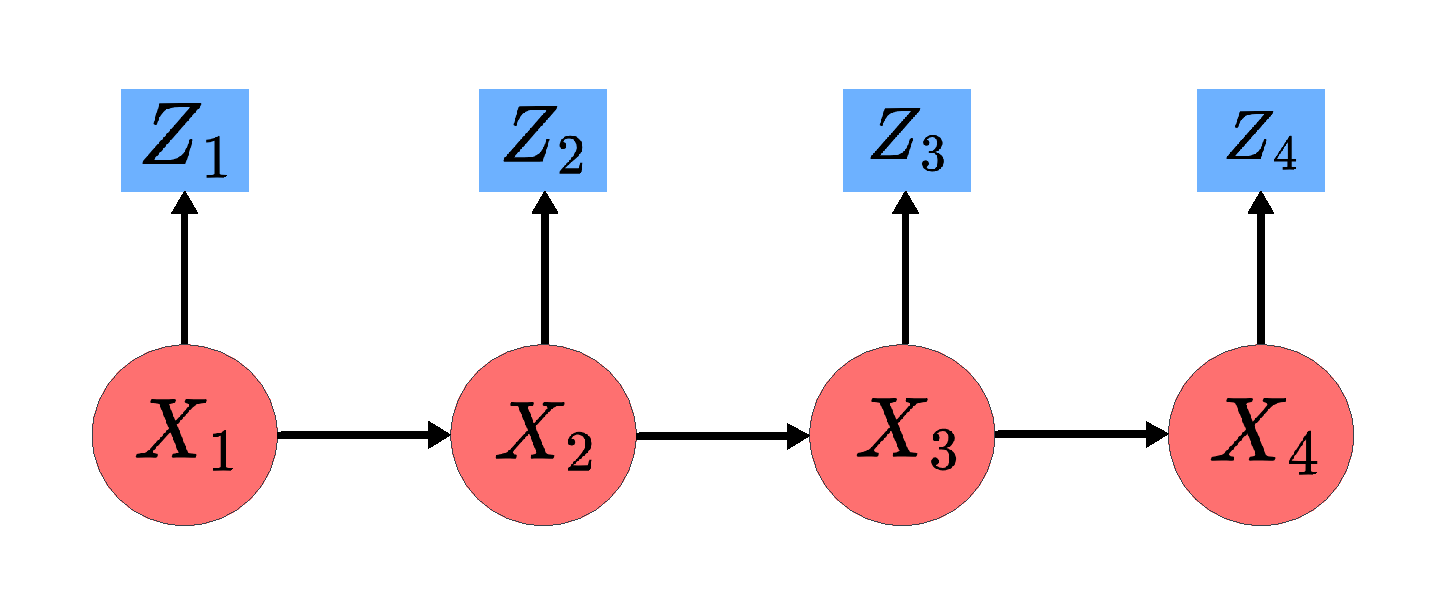
\includegraphics[width=0.5\linewidth]{img/BeyseNetAppendix}
	\caption{شبکه بیز معادل مربوط به مسئله مثال  تخمین حالت بیان‌شده}
	\label{fig:beysenetappendix}
\end{figure}

فرمول‌بندی احتمالاتی بیزی که تا کنون ذکر شده است، می‌تواند به صورت گرافیکی
با استفاده از شبکه‌های بیزی ارائه شود. یک شبکه بیزی
\footnote{\lr{BayesNet}}
یک مدل گرافیکی جهت‌دار است
که متغیرهای تصادفی به عنوان گره‌های آن و یال‌ها نمایانگر وابستگی‌ها (علت و معلول)
بین این گره‌ها هستند. به عبارت دیگر، یک شبکه بیزی می‌تواند توزیع احتمالی مشترک
را بر روی همه متغیرهای تصادفی به عنوان حاصل‌ضرب چگالی‌های شرطی تعریف کند. شکل~\ref{fig:beysenetappendix}
شبکه بیزی مربوط به سیستم غیرخطی مثال ما را نشان می‌دهد. توزیع احتمالی مشترک
مربوطه ممکن است به صورت زیر نوشته شود:
\begin{equation} \label{eq:JointProbability_Distribution}
	p(X, Z) = p(x_1) p(x_2|x_1) p(x_3|x_2) p(x_4|x_3) \newline
	\times p(z_1|x_1) p(z_2|x_2) p(z_3|x_3) p(z_4|x_4)
\end{equation}
در این معادله، تکه اول اول نمایانگر مدل سیستم و تکه دوم
نمایانگر مدل‌های مشاهده است.

 توزیع مشترک در معادله
 \ref{eq:MAP}
 به توزیع پسین \(p(X|Z)\) با استفاده از فرمول احتمال شرطی زیر پیوند می‌خورد:
\begin{equation}
	p(X|Z) = \frac{p(X, Z)}{p(Z)}
\end{equation}
\(p(Z)\) در این معادله به عنوان یک عامل نرمال‌سازی عمل می‌کند، بنابراین \(p(X|Z)\) متناسب با توزیع مشترک \(p(Z, X)\) است. تخمین $MAP$ معادل خواهد بود با بیشینه‌سازی تابع درست‌نمایی \(l(X; Z)\) که متناسب با \(p(Z, X)\) است:
\begin{equation}
	l(X; Z) \propto p(Z|X)
\end{equation}
بدین‌ترتیب خواهیم داشت:
\begin{equation}
	X^{MAP} = \arg\max_X l(X; Z)
\end{equation}
علاوه بر این، می‌توانیم مقیاس‌های ثابت را در احتمالات شرطی معادلات
\ref{eq:Gauess_Dis_h}
و
\ref{eq:Gauess_Dis_F}
حذف کنیم و تابع درست‌نمایی \(l(X; Z)\) را به صورت زیر بنویسیم:
\begin{equation} \label{eq:Likelihood}
	l(X; Z) = l(x_1) l(x_2|x_1) l(x_3|x_2) p(x_4|x_3) \\
	\times l(z_1|x_1) l(z_2|x_2) l(z_3|x_3) l(z_4|x_4)
\end{equation}
که در آن:
\begin{equation}
	l(X; z) = \exp \left\{ -\frac{1}{2} \|g(X) - z \|_R^2 \right\}
\end{equation}
\begin{equation}
	l(X_{k+1}; X_k) = \exp \left\{ -\frac{1}{2} \|f(X_k, u_k) - X_{k+1}\|_Q^2 \right\}
\end{equation}

\begin{figure} [!t]
	\centering
	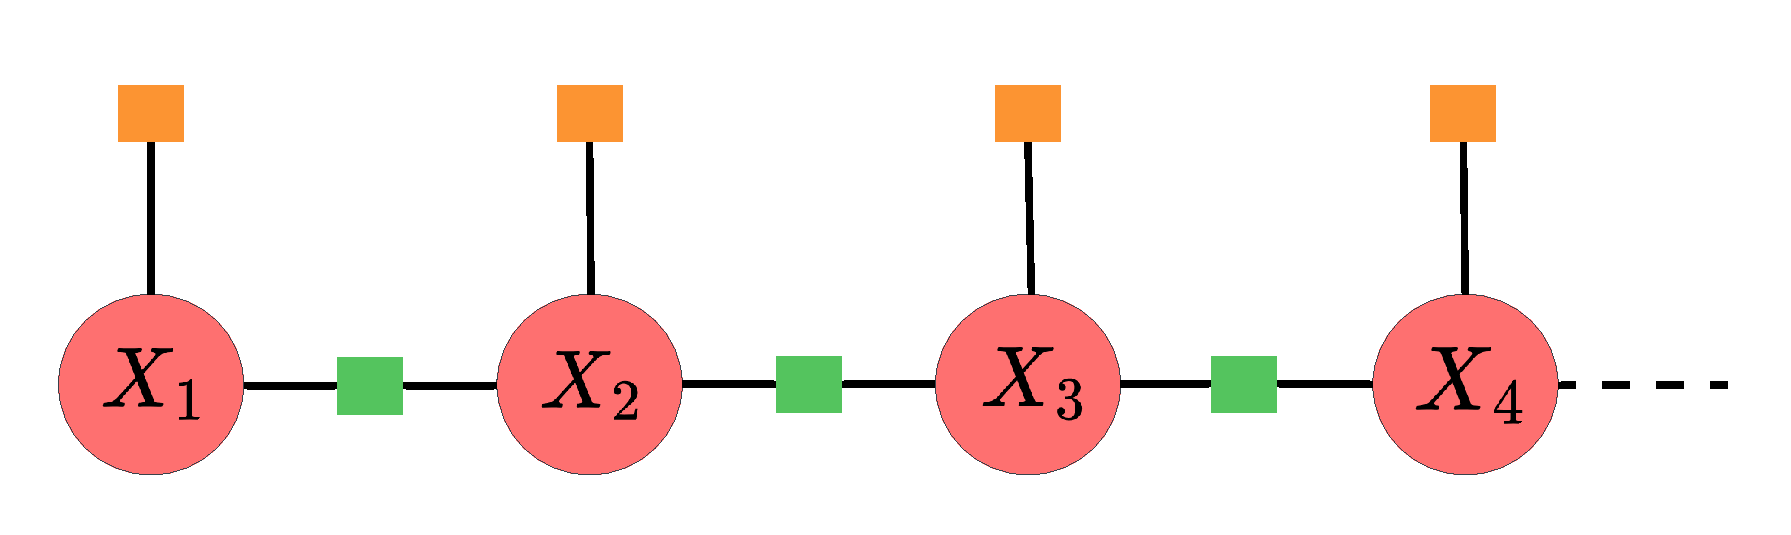
\includegraphics[width=0.6\linewidth]{img/StateEstimationFGAppendinx}
	\caption{گراف عامل معادل مربوط به مسئله مثال  تخمین حالت بیان‌شده}
	\label{fig:stateestimationfgappendinx}
\end{figure}

بنابراین، تابع درست‌نمایی که باید بیشینه شود، حاصل‌ضرب تجزیه‌شده‌ای از توابع درست‌نمایی کوچکتر است. در حالی که توزیع احتمالی مشترک در معادله
\ref{eq:JointProbability_Distribution}
به بهترین شکل با استفاده از یک شبکه بیزی توصیف می‌شود، تابع درست‌نمایی تجزیه‌شده در معادله
\ref{eq:Likelihood}
می‌تواند به بهترین شکل با یک گراف عامل نمایش داده شود.

یک گراف عامل \(G\) تجزیه یک تابع \(f(X)\) را به عنوان حاصل‌ضربی از عامل‌های \(f_i\) تعریف می‌کند. این یک مدل گرافیکی دو بخشی و بدون جهت با دو نوع گره است: گره‌های عامل \(f_i \in F\) و گره‌های متغیر \(x_i \in X\). یک یال \(e_{ij} \in E\) در گراف حضور دارد اگر و فقط اگر \(f_i\) تابعی از \(x_j\) باشد
\cite{kaess2012concurrent}. 
شکل
\ref{fig:stateestimationfgappendinx}
گراف عامل متناظر با تابع درست‌نمایی در معادله
\ref{eq:Likelihood}
را نشان می‌دهد. در این شکل، عامل‌های آبی رنگ به درست‌نمایی‌های اندازه‌گیری اشاره دارند در حالی که عامل‌های سبز رنگ به مدل سیستم اشاره می‌کنند.
در نهایت، با استفاده از الگوریتم $ML$، مسئله $MAP$ به یک مسئله $LS$ غیرخطی زیر تبدیل می‌شود:
\begin{equation}
	X^{MAP} = \arg\max_X l(X; Z) = \arg\max_X \text{Ln}\left(\prod_i l_i (X_i; Z_i)\right)
\end{equation}
\begin{equation}
    X^{MAP}	= \arg\min_X \left(\sum_{i=0}^k \left(\|f(x_i, u_i) - x_{i+1}\|_{Q_i}^2 + \|h(x_i) - z_i\|_{R_i}^2\right)\right)
\end{equation}

در مورد سیستم‌های ناوبری، \(X\) نشان‌دهنده مکان‌های پیگیری شده است که از طریق عامل‌های مدل حرکت به یکدیگر متصل می‌شوند. از طرف دیگر، هر حالت نیز با فاکتورهای مدل اندازه‌گیری محدود می‌شود.

\section{حل‌کننده‌ها}

راه‌حل یک مسئله $LS$ که به یک گراف عامل مربوط است، می‌تواند به چهار روش تقسیم شود. در ادامه، این چهار روش معرفی می‌شوند.

\textbf{بهینه‌سازهای دسته‌ای}

در بهینه‌سازی دسته‌ای، همه عامل‌ها از ابتدای زمان تا لحظه فعلی در الگوریتم بهینه‌سازی شرکت می‌کنند. از آنجا که تمام اطلاعات در مسئله بهینه‌سازی شرکت می‌کنند، این روش دقیق‌ترین نتیجه را به دست می‌دهد. با این حال، به دلیل بار محاسباتی سنگین، این یک الگوریتم آفلاین است.

\textbf{فیلترها و صاف‌کننده‌های با تأخیر ثابت}

بهینه‌سازهای دسته‌ای با گذشت زمان در پیچیدگی رشد می‌کنند، بنابراین اجرای آن‌ها در زمان واقعی غیرممکن خواهد بود. بنابراین، یک راه‌حل این است که اطلاعات قدیمی را با حاشیه‌نویسی حذف کنیم و اثر تجمعی آن‌ها را به عنوان یک عامل پیشین در انتهای گراف عامل بریده‌شده اضافه کنیم. این حاشیه‌نویسی و برش در هر تکرار الگوریتم رخ می‌دهد. مقیاس مسئله در این حالت ثابت می‌ماند و به اندازه پنجره بستگی دارد.

در فیلتر کردن، که یک حالت شدید از صاف کردن با تأخیر ثابت است، همه داده‌های قبلی تا گره فعلی به یک عامل پیشین واحد فشرده می‌شوند. این حالت کمترین سربار محاسباتی و ذخیره‌سازی را دارد. اگرچه این برش گراف عامل برای سیستم‌های خطی هیچ اثر تباه‌کننده‌ای ندارد، اما برای سیستم‌های غیرخطی، منجر به تجمع خطاها در عامل پیشین می‌شود. این تجمع به دلیل اصلاح نقاط خطی‌سازی در هر تکرار است که دیگر نمی‌توانند به گره‌های قبلی منتقل شوند.

\textbf{صاف‌کننده‌های افزایشی}

صاف کردن افزایشی که در
\cite{kaess2012concurrent}
ارائه شده است، یک الگوریتم جدید برای افزودن افزایشی و حل گراف عامل به صورت افزایشی با ورود داده‌های جدید است. از آنجا که مسائل تخمین حالت در رباتیک معمولاً به یک زنجیره مارکوف منجر می‌شوند، گراف فاکتور تولید شده اغلب تنک است و تجزیه ماتریس مورد نیاز در طی اجرای بهینه‌سازی غیرخطی تکراری می‌تواند به صورت کارآمدتری انجام شود. نویسندگان در
\cite{kaess2012concurrent}
از روش‌های تجزیه ماتریس تکراری برای توسعه الگوریتم خود بهره‌برداری می‌کنند.

به دلیل ماهیت مارکوفی مسئله، شبکه بیزی تولید شده یک گراف وتری
\footnote{\lr{chordal graph}}
 است. این گراف وتری سپس به یک درخت بیزی تبدیل می‌شود. ممکن است اطلاعات جدید به‌راحتی اضافه شوند بدون نیاز به اجرای مجدد تمام محاسبات. با اینکه زمان محاسباتی این روش بسیار کمتر است، نیازهای حافظه تغییر نمی‌کنند. علاوه بر این، نمی‌توان مطمئن بود که هر تکرار از این الگوریتم چقدر زمان خواهد برد. بنابراین، به‌طور کلی، این روش نمی‌تواند تخمین‌های قطعی ارائه دهد، و بر اساس مسئله و اندازه‌گیری‌های مشاهده‌شده، زمان محاسباتی ممکن است به‌طور قابل‌توجهی متفاوت باشد. به عنوان مثال، وقتی یک محدودیت حلقه اضافه می‌کنیم، تکرار جدید نیاز دارد تا بخش بیشتری از درخت پردازش شود، که نیازمند زمان محاسباتی بسیار بیشتری است.

\textbf{فیلتر کردن و صاف کردن همزمان}

مقاله
\cite{kaess2012concurrent}
یک چارچوب با یک فیلتر در حال اجرا در کنار یک صاف‌کننده ارائه می‌دهد. در هر تکرار صاف‌کننده، فیلتر می‌تواند چندین بار تکرار شود و تخمین‌های بلادرنگ ارائه دهد. سپس، در انتهای هر تکرار صاف‌کننده، این دو سیستم هماهنگ می‌شوند. جداسازی این دو سیستم از طریق یک متغیر جداکننده میانی در درخت بیزی به دست می‌آید. با داشتن این متغیر، فیلتر از لحاظ آماری از صاف‌کننده مستقل خواهد بود. در مرحله همگام‌سازی، جداکننده به‌روزرسانی می‌شود به طوری که حالت‌های جدیداً اضافه‌شده به فیلتر به درخت صاف‌کننده منتقل شوند.

\section{کتابخانه GTSAM}

همان‌طور که در بخش‌های قبلی ذکر شد، گراف‌های عامل ابزارهای قدرتمندی برای فرمول‌بندی مسائل تخمین حالت و کالیبراسیون هستند. به دلیل انعطاف‌پذیری آن‌ها، این گراف‌ها به روشی کارآمد برای ساخت مسائل بهینه‌سازی نقشه در سیستم‌های SLAM تبدیل شده‌اند. بنابراین، بسیاری از
حل‌کننده‌های متن‌باز و کارآمد برای پیاده‌سازی این ابزار توسعه داده شده‌اند. یکی از کتابخانه‌های
مهم، GTSAM 
\cite{gtsam}
است. این کتابخانه در دانشگاه جورجیاتک توسعه یافته و یک رابط برنامه‌نویسی کامل برای پیاده‌سازی عامل‌های سفارشی، تعریف گراف‌های عامل، و حل آن‌ها به‌صورت کارآمد فراهم می‌کند.

علاوه بر این، GTSAM از بهینه‌سازی روی منیفلدها نیز پشتیبانی می‌کند، که در مواردی که با مسائل بهینه‌سازی مواجه هستیم که به پارامترهایی از گروه‌های اقلیدسی خاص مربوط می‌شوند، ضروری است. این کتابخانه همچنین یک رابط نرم‌افزار متلب برای توسعه سریع ارائه می‌دهد. در نهایت، بسیاری از عامل‌ها که قبلاً در این کتابخانه پیاده‌سازی شده‌اند، آماده بهره‌برداری برای مسائل رباتیک و SLAM هستند.